\documentclass[tikz,border=7pt]{standalone}
\usepackage[T1]{fontenc}
\usepackage{lmodern,graphicx}
\usetikzlibrary{arrows.meta}
\definecolor{navy}{HTML}{17334F}
\definecolor{teal}{HTML}{176E68}
\definecolor{muted}{HTML}{52616D}
\begin{document}
\sffamily
\begin{tikzpicture}[text=navy,>=Stealth]
\node[font=\large\bfseries] at (6,1.35) {Hand landmark recovery through image preprocessing};
\draw[navy,line width=.7pt] (-2.3,.85)--(14.3,.85);
\foreach \x/\n/\heading in {0/1/Original detection,6/2/Image preprocessing,12/3/Detection retry}{
 \node[font=\normalsize\bfseries] at (\x,.35) {\n\quad\heading};
}
\node at (0,-1.65) {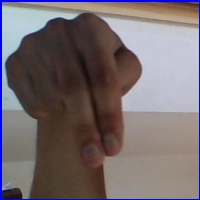
\includegraphics[width=31mm]{N47_original.png}};
\node at (6,-1.65) {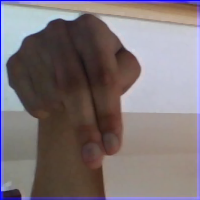
\includegraphics[width=31mm]{N47_dilated.png}};
\node at (12,-1.65) {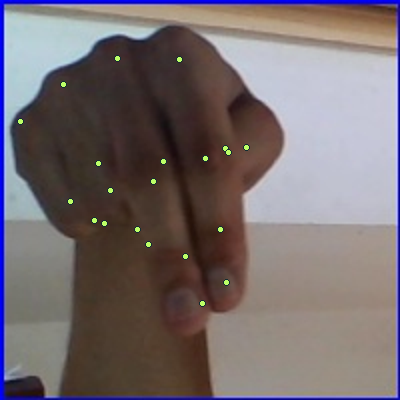
\includegraphics[width=31mm]{N47_overlay.png}};
\draw[->,navy,line width=1pt] (2,-1.65)--(3.9,-1.65);
\draw[->,navy,line width=1pt] (8,-1.65)--(9.9,-1.65);
\node[align=center,font=\small,text width=44mm] at (0,-4.05)
 {Original N47\\MediaPipe returns \texttt{no\_hand}};
\node[align=center,font=\small,text width=44mm] at (6,-4.05)
 {Square \(3\times3\) dilation\\One application to the colour image};
\node[align=center,font=\small,text width=44mm] at (12,-4.05)
 {MediaPipe returns \texttt{ok}\\Recovered points on original pixels};
\draw[teal,line width=.6pt] (-2.3,-4.8)--(14.3,-4.8);
\node[font=\small,text=muted,align=center] at (6,-5.3)
 {Both detection attempts use the same model and confidence thresholds (0.50).\\
 N47 is a development example; landmark plausibility requires visual assessment.};
\end{tikzpicture}
\end{document}
